\documentclass{article}

\usepackage[%
    left=0.5in,%
    right=0.5in,%
    top=0.5in,%
    bottom=0.5in,%
]{geometry}%
\usepackage{minitoc}
\usepackage{multicol}
\usepackage{graphicx}
\usepackage{fixltx2e}
\usepackage{listings}
\usepackage{color}
\usepackage{hyperref}
    \hypersetup{ colorlinks = true, linkcolor = blue }
\usepackage{blindtext}
\definecolor{lightgray}{gray}{0.9}
\graphicspath{ {./} }

\newcommand{\inlinecode}[2]{\colorbox{lightgray}{\lstinline
[language=#1]$#2$}}
\newcommand{\worddef}[1]{\hyperref[sec:reference]{\textit{#1}}}

\begin{document}

\tableofcontents

\newpage

\section{Architecture}

\begin{multicols}{2}
\begin{itemize}
  \item A software stack for mobile devices
  \item Operating system kernel
  \item Standard middleware
  \begin{itemize}
    \item Android library support
  \end{itemize}
  \item Key applications / user interfaces
  \begin{itemize}
    \item Vendor specific modifications
  \end{itemize}
  \item LK: threading, low level memory management, driver
  \item HAL: libs for hardware module
  \item AR: virtual machine
  \item NCL: fundamental core functionalities
  \item API: programming interface
  \item APP: system apps can be customised.
\end{itemize}

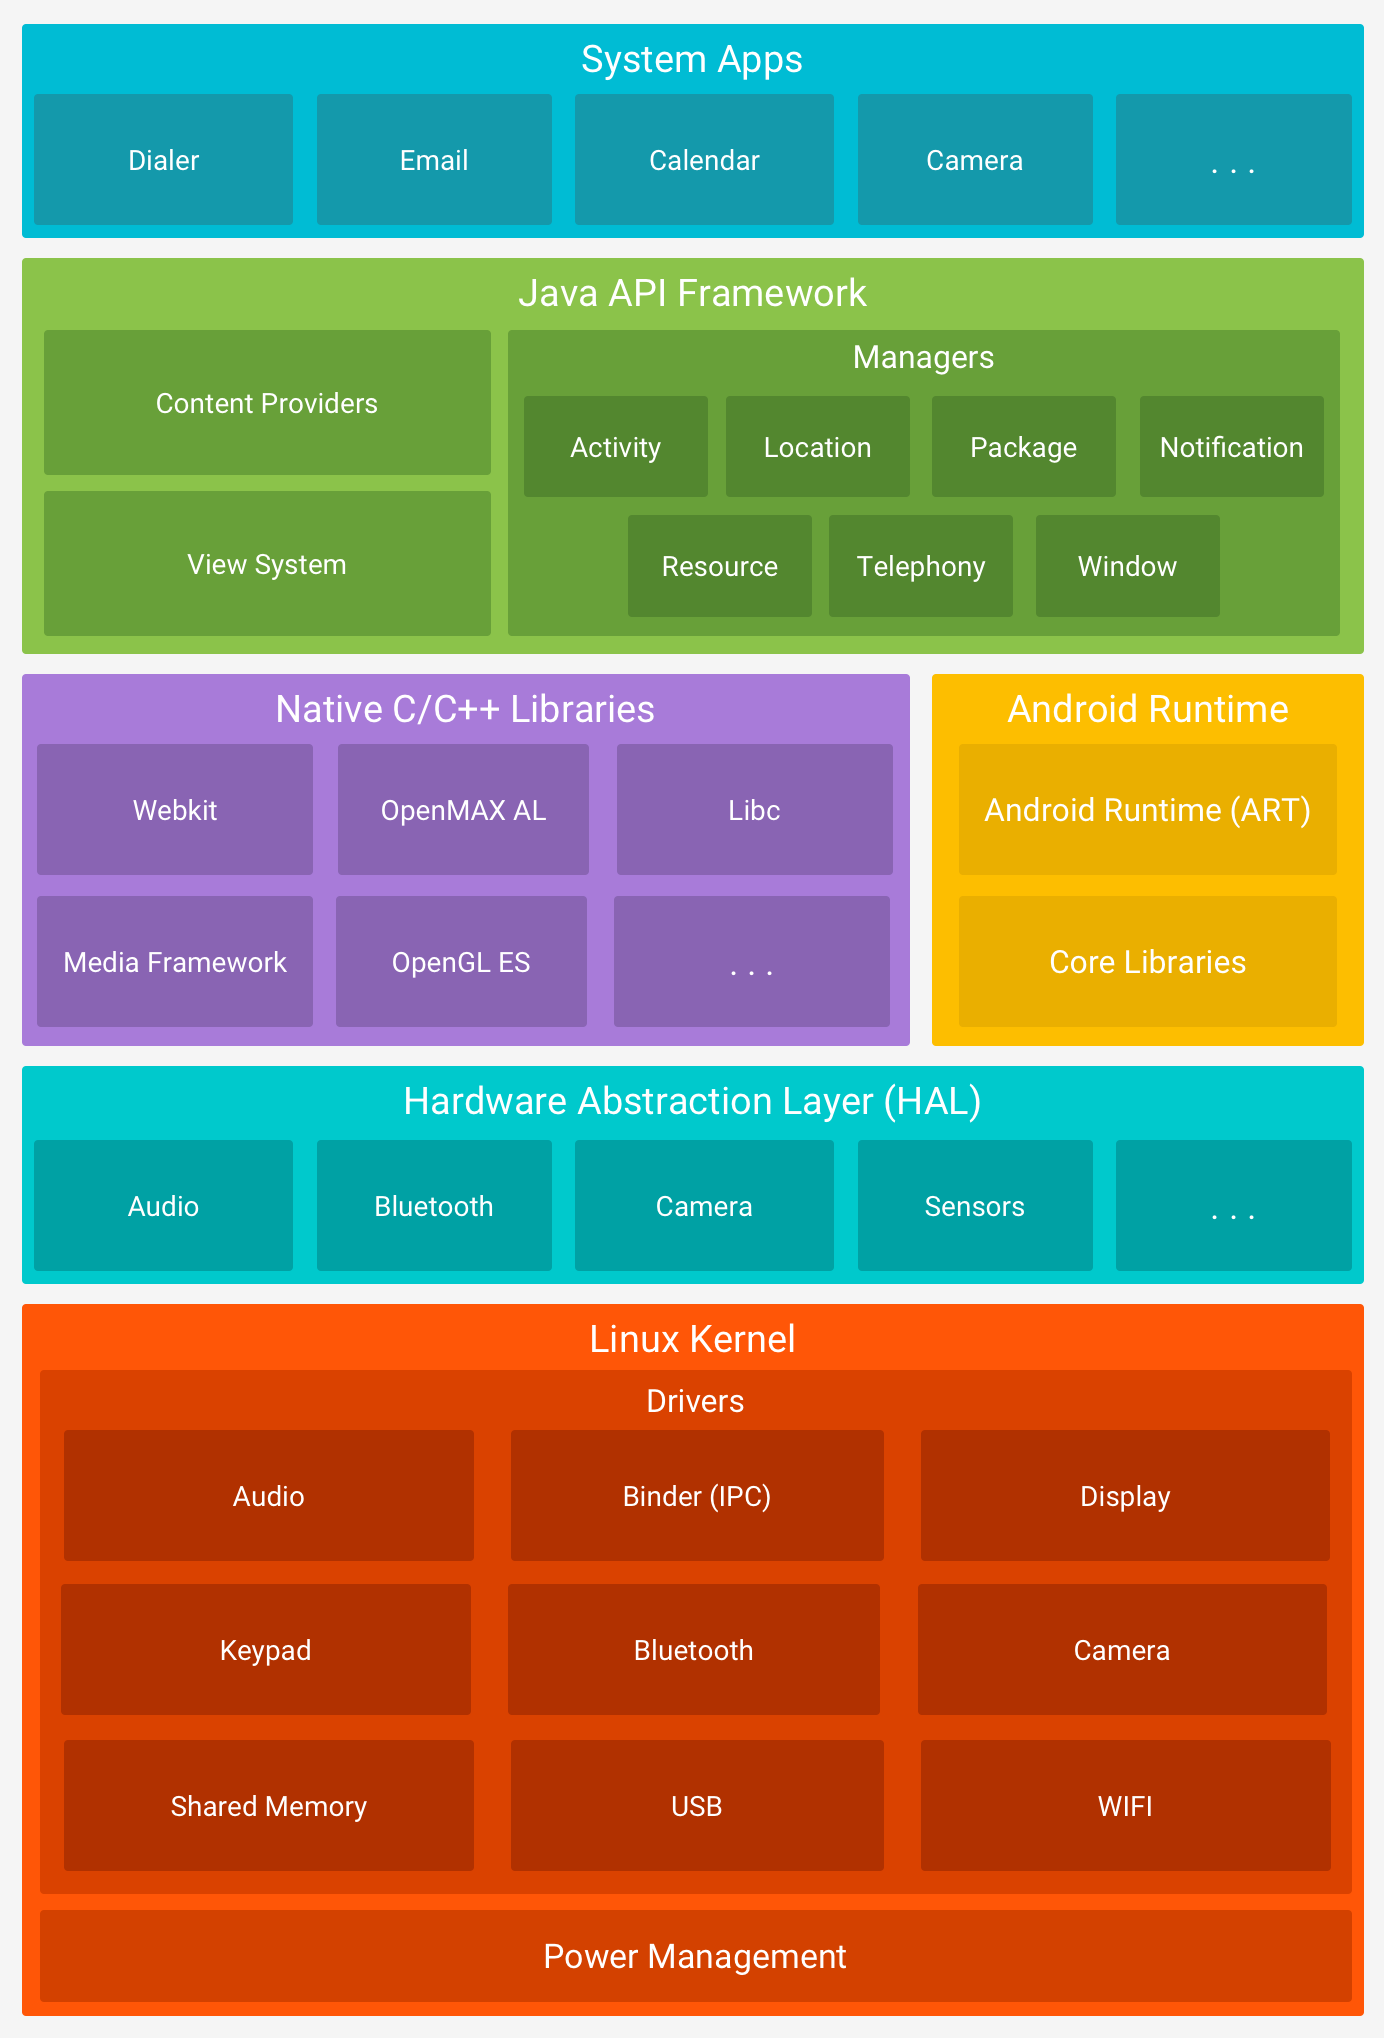
\includegraphics[scale=0.1]{android-stack_2x.png}

\end{multicols}

\subsection{Kernel}

\begin{multicols}{2}

\subsubsection{Modifications}

\begin{flushleft}
  Modifications made by android to linux OS
\end{flushleft}
\begin{itemize}
  \item wakelocks
  \begin{itemize}
  	\item Keep the phone awake
  \end{itemize}
  \item binder
  	\begin{itemize}
  		\item Interprocess communication mechanism, and remote method invocation system.
  		\item One Android process can call a routine in another Android process
  	\end{itemize}
  \item ashmem
  \begin{itemize}
  	\item Android Shared Memory
  	\item A component of the Android operating system that facilitates memory sharing and conservation
  \end{itemize}
  \item oom – kills processes when memory is low
  \item alarm manager
  \begin{itemize}
  	\item Wakes up the phone when necessary
  \end{itemize}
\end{itemize}

\vfill\null

\subsection{Hardware support}
\begin{itemize}
  \item Bluetooth - BlueZ
  \item GPS – Manufacturer provided libgps
  \item Wifi – \texttt{wpa-supplicant}
  \item Display – Standard framebuffer driver
  \item Keyboard – Standard input event
  \item Lights – Manufacturer provided liblights.so
  \item Audio – Manufacturer provided libaudio.so
  \item Camera – Manufacturer provided libcamera.so
  \item Power Management – “wakelocks” kernel patch
  \item Sensors – Manufacturer provided libsensors.so
  \item Radio – Manufacturer provided libril.so
\end{itemize}

\end{multicols}

\subsection{Security}

Applications are sandboxed
\begin{itemize}
 \item A security mechanism for separating running applications and data
 \item This allows applications run in a different context, so if one app crashed, others can stay uneffected
 \item On Android, each app runs as its own \textbf{user}, which guarantees that different users are unable to interfere with each other, access each other’s files and so on. Root can access the entire system
 \item Own process, own VM, own UID/AID for different app
\end{itemize}

\newpage

\section{System boot process}

\begin{multicols}{2}
  \begin{itemize}
		\item \textbf{Boot ROM/ Bootloader:} Load bootloader into RAM, detect external RAM, setup network, memory, etc.
		\item \textbf{Kernel:} Setup cache, protected memory, scheduling and loads drivers.
		\item \textbf{Init:} Mounts directories like /sys , /dev or /proc Runs init.rc script
		\item \textbf{Zygote \& VM:} Enables code sharing across the android VM for quick start of separate VM for different apps preloadClasses(), preloadResources()
		\item \textbf{System service:} Power manager, activity manager, telephony registry, package manger, context manager, system contact providers, etc.
	\end{itemize}
	\vfill\null

	\begin{center}
	  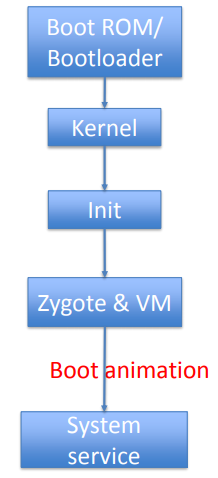
\includegraphics[scale=0.5]{boot_process.png}
	\end{center}
\end{multicols}

\section{Zygote}
\begin{itemize}
  \item Initialised process that has all core libraries linked in
  \item Load all java.*, android.* classes at boot time
  \item Initially create a single android VM process – Referencing classes loaded above
  \item When user runs an application:
  \begin{itemize}
    \item Creates a copy of itself in a separate address space
    \item \textbf{Does not} copy memory, instead refers to original memory until modified
    \item Because each container recieves a map, these resources are shared between applications, eliminating the need for each new fork of the VM to keep its own copy of classes and resource.
  \end{itemize}
\end{itemize}

\section{Memory}
\begin{flushleft}
In many places, Android shares the same dynamic RAM across processes using explicitly allocated shared memory regions.
Android uses paging and mmap instead of providing swap space, which means any memory your application touches cannot be paged out unless you release all references.
\end{flushleft}

\section{Android compilation}

\newpage

\begin{description}
	\item[placeholder] \hfill \\
\end{description}
\end{document}
